\chapter{Results}
\label{chap:results}

\section{Introduction}

In the previous chapter, we described the parameters of a commercial WDM optical fiber communication system with a frequency signal that is located between two data channels, as shown in Fig.~\ref{fig:system}. Given reasonable system parameters, we showed that the dominant optical impairment is XPM, given by Eq.~\ref{eq:phasedistort}, and all other optical impairments can be made negligible.

It follows that the phase distortion depends on the length of fiber, the frequency separation between the frequency signal and the data channels, and the power of the neighboring data channels as they change over the course of their propagation. We will now vary these parameters and investigate their effect on the stability of the frequency signal.

We choose a value for the data channel power that is typical in commercial optical communication systems. These values are chosen to minimize nonlinear distortion in the data signals \cite{Agrawal2013, agrawal2012fiber}. Hence, we neglect the nonlinear distortion of the data signals when calculating $\phi(z,t)$ and focus on the effect of dispersion. The evolution of the data signal is then easily obtained in the Fourier domain, and we find
%
\begin{equation} \label{eq:datasol}
u_d(z,T) = \frac{1}{2\pi} \int_{-\infty}^{\infty} U_d(0, \omega')\exp\left(-\frac{\alpha}{2} z + i\delta\omega' z + \frac{i}{2}\beta_2\omega'^2z-i\omega' T\right) d\omega' ,
\end{equation}
%
where $U_d(0,\omega)$ is the Fourier spectrum of the data signal at $z=0$, defined as
\begin{equation}
U_d(0,\omega) = \int_{-\infty}^{\infty} u_d(0, t')\exp(i\omega t')dt'.
\end{equation}

We begin by investigating the distribution of the power of the data signal $|u_d|^2$ as a function of length $z$. The on-off-keyed, nonreturn-to-zero (OOK-NRZ) symbols of the data signal change over the length of the fiber due to dispersion, self-phase modulation, and attenuation. We first study a system in which attenuation is neglected. We then add the effect of attenuation. Finally, we study the system behavior as the group velocity difference due to the frequency separation between the neighboring data channels and frequency signal increases.

\section{Simulation Parameters}

The simulated data signal is a $2^{10}-1$ pseudorandom binary sequence (PRBS) \cite{PRBS} that is OOK-NRZ modulated with optical power of $1$ mW with periodic boundary conditions. A PRBS has properties that resemble a random sequence. It is approximately delta-correlated, and has an almost equal number of $0$s and $1$s. As a consequence, the statistical properties of the signal converges more rapidly as the sequence length increases than if the string of $0$s and $1$s are randomly chosen. PRBS signals are commonly used in both computer simulations and laboratory experiments to model data channels. The length of the string is chosen so that the string does not repeat as the data channel travels through a fixed time point in the frequency signal.

The fiber has an attenuation of $\alpha = 0.2$ dB/km, group velocity dispersion $\beta_2 = -22$ ps$^2$/km, and Kerr nonlinearity $\gamma = 1.3$ W$^{-1}$km$^{-1}$. The data signal has a central wavelength of $1530$ nm with inverse group velocity difference $\delta = 1$ ps/km relative to the frequency signal. These parameters are typical for optical fiber communication systems \cite{agrawal2012fiber,Agrawal2013}. We will vary some of these parameters in the following sections as we study the changes in the XPM-induced phase distortion.


\section{Without Attenuation}

We first neglect attenuation in order to provide a baseline against which to determine its effect.

During propagation, the optical power in each bit of the data signal spreads outside of its time slot into the time slots of its neighbors. After some long distance, the expected power in each time slot will become the same. Therefore, the variance of the data signal's optical power is expected to decrease as a function of fiber length, although there will be statistical fluctuations in the pseudo-random signal that we are using. Figure~\ref{fig:NACalcVar} shows the data signal power variance as the distance varies up to $800$ km. Since there is no attenuation, the mean of the data signal power is constant. Though not shown in the figure, longer propagation distances yield a variance on the order of $1.8 \times 10^{-7}$ W$^2$.
%
\begin{figure}[htb]
	\raggedright
	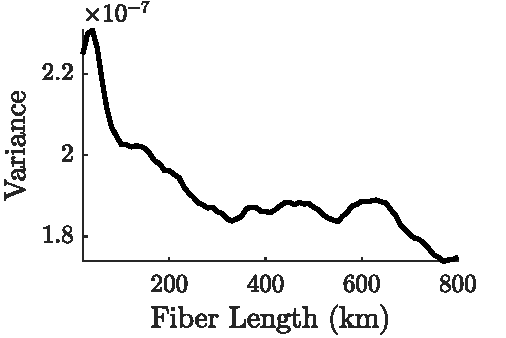
\includegraphics[scale=0.8]{img/NACalcVar}
	\renewcommand{\baselinestretch}{1}
	\small\normalsize
	\caption{Data channel optical power variance vs. fiber length.} \label{fig:NACalcVar}
\end{figure}
\renewcommand{\baselinestretch}{2}
\small\normalsize

The phase shift $\phi$ grows as a function of distance because the frequency signal experiences cross-talk from the data signal, which accumulates over the propagation length. Figures \ref{fig:NAPhiMean}a and \ref{fig:NAPhiVar}b show the mean and variance of the phase shift of the frequency signal due to XPM. The mean of $\phi$ grows linearly with respect to the fiber length because without attenuation the average energy in the data signal is constant. As a consequence, the mean additive phase error can be compensated.
%
\begin{figure}[htb]
	\raggedright
	\begin{tabular}{c c}
		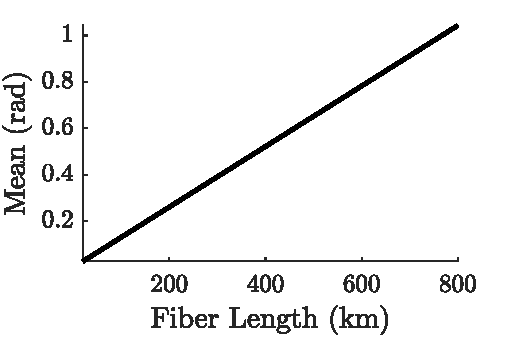
\includegraphics[width=0.5\linewidth]{img/NAPhiMean} & 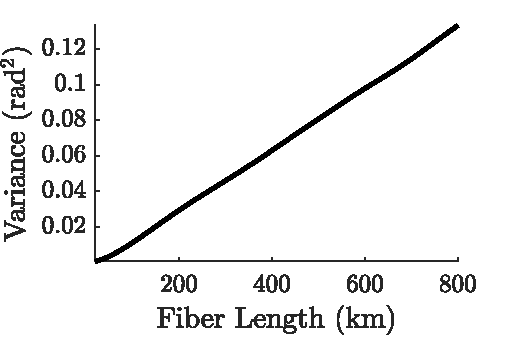
\includegraphics[width=0.5\linewidth]{img/NAPhiVar} \\
		(a) & (b)
	\end{tabular}
	\renewcommand{\baselinestretch}{1}
	\small\normalsize
	\caption{(a)\label{fig:NAPhiMean} Mean of $\phi$ vs. fiber length (b)\label{fig:NAPhiVar} Variance of $\phi$ vs. fiber length.}
\end{figure}
\renewcommand{\baselinestretch}{2}
\small\normalsize

We now quantify the phase deviation using the measures that we introduced in Chapter \ref{chap:time_stability}. We first consider the first structure equation, $D^{(1)}_\phi = \langle [\phi(t+\tau) - \phi(t)]^2 \rangle$, which represents the mean phase accumulation. As we discussed in Chapter \ref{chap:time_stability}, the structure functions are related to the autocorrelation function. A typical data signal is a collection of apparently random bits that are uncorrelated with each other. As the data signal propagates through the fiber, the optical energy associated with each bit occupies a larger amount of time due to dispersion, so that the amount of time in which a bit is correlated with itself increases. Figure \ref{fig:NAPhaseStability} shows $\left[D^{(1)}_\phi\right]^{1/2}$ at different lengths. The phase deviation becomes constant after a short amount of time.

Figure \ref{fig:NAAllanDev} shows the Allan deviation. After averaging the fractional frequency over a time interval on the order of the duration of the bit pulse, $\tau = 10^{-10}$ s, the Allan deviation starts to fall off at a rate proportional to $\tau^{-1}$. This falloff signifies that rapidly oscillating errors are being averaged out. We expect the falloff to continue indefinitely because XPM contributes no long-term frequency drift. We have computed the Allan deviation up to $10$ ns, at which point the trend proportional to $\tau^{-1}$ is apparent. Extrapolating the $\tau^{-1}$ dependence to longer averaging times, we find that the Allan deviation is $3\times 10^{-15}$ at $\tau = 1$ s, and $3\times 10^{-18}$ at $\tau=10^3$ s.

%
\begin{figure}[htb]
	\raggedright
	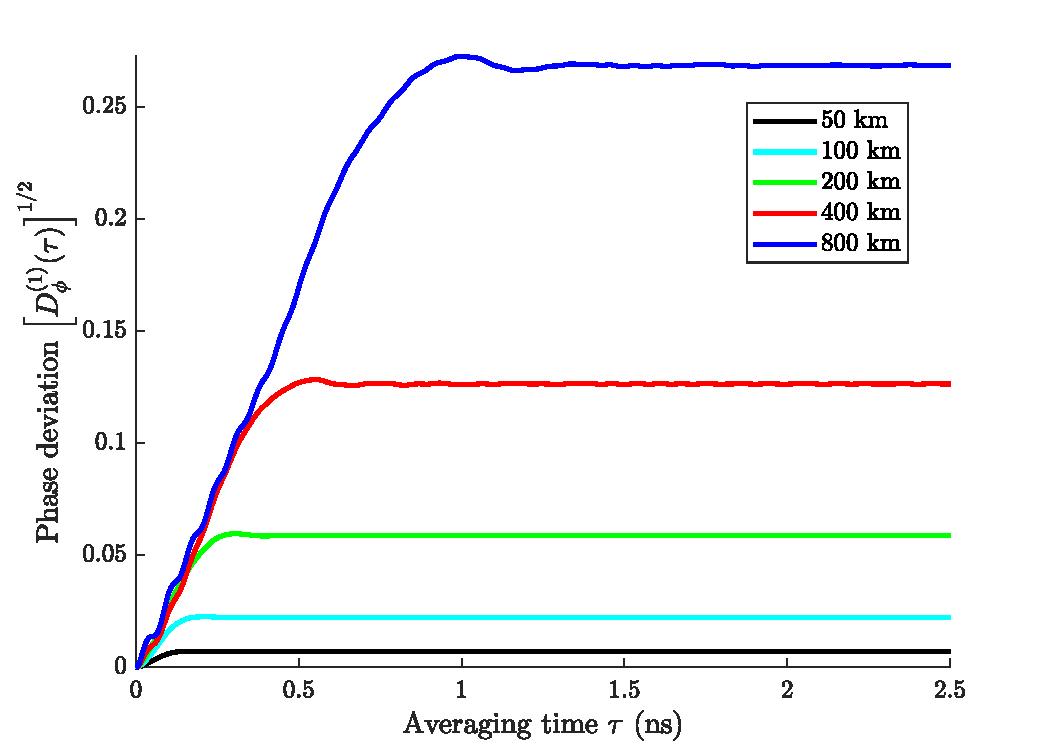
\includegraphics[scale=0.8]{img/NAPhaseStability}
	\renewcommand{\baselinestretch}{1}
	\small\normalsize
	\caption{Phase deviation without attenuation.} \label{fig:NAPhaseStability}
\end{figure}
\renewcommand{\baselinestretch}{2}
\small\normalsize

%
\begin{figure}[htb]
	\raggedright
	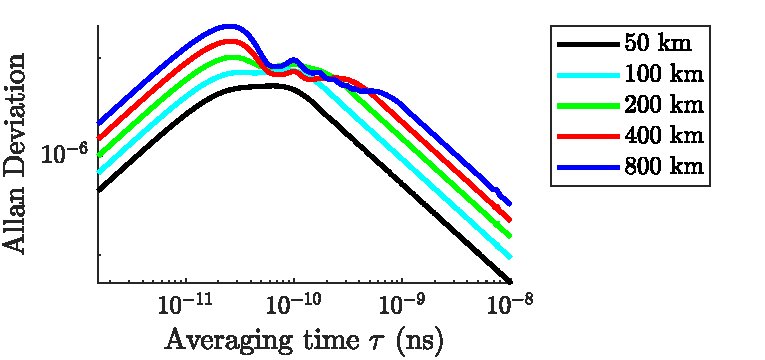
\includegraphics[scale=0.8]{img/NAAllanDev}
	\renewcommand{\baselinestretch}{1}
	\small\normalsize
	\caption{Allan deviation without attenuation.} \label{fig:NAAllanDev}
\end{figure}
\renewcommand{\baselinestretch}{2}
\small\normalsize

\clearpage

\section{Effect of Attenuation}

We now include the effect of attenuation. We expect the phase and frequency instability to be lower than was the case without attenuation because the effective length before the nonlinearity and hence XPM become negligible is $20$ km after each amplifier.

%
\begin{figure}[htb]
	\raggedright
	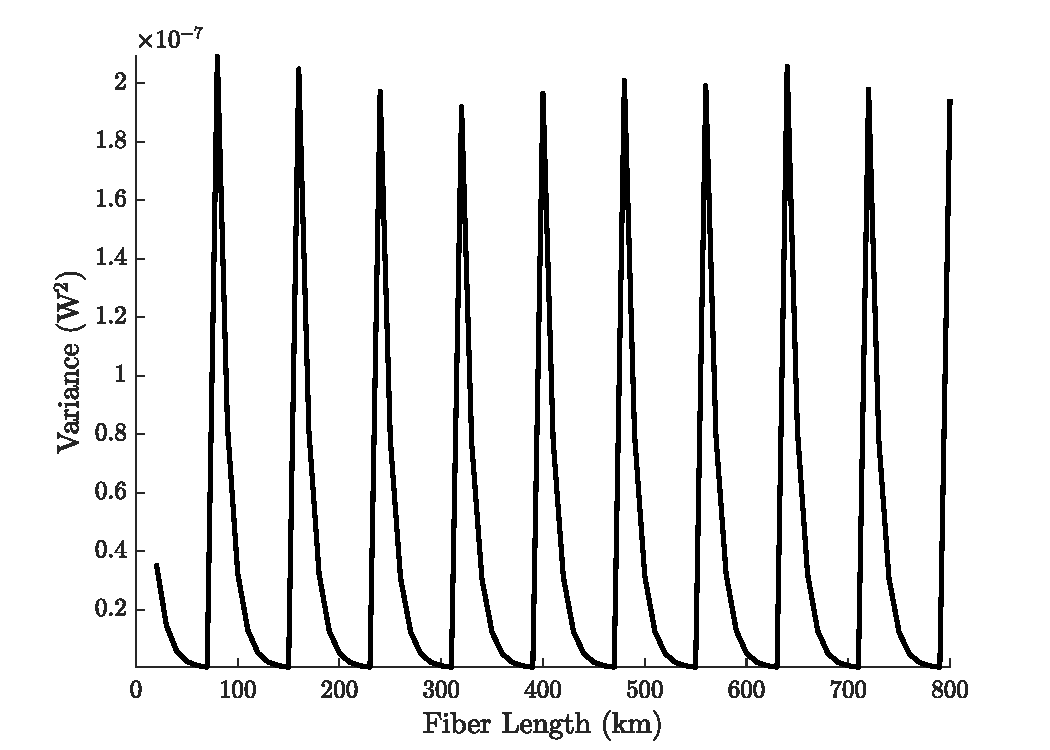
\includegraphics[scale=0.8]{img/ACalcVar}
	\renewcommand{\baselinestretch}{1}
	\small\normalsize
	\caption{Data channel optical power variance vs. fiber length.} \label{fig:ACalcVar}
\end{figure}
\renewcommand{\baselinestretch}{2}
\small\normalsize

First, we compare the variance of the attenuated data signal with the variance without attenuation. Figure~\ref{fig:ACalcVar} shows the data signal's optical power variance. Spikes occur every $80$ km, corresponding to the locations of the amplifiers.

%
\begin{figure}[htb]
	\raggedright
	\begin{tabular}{c c}
		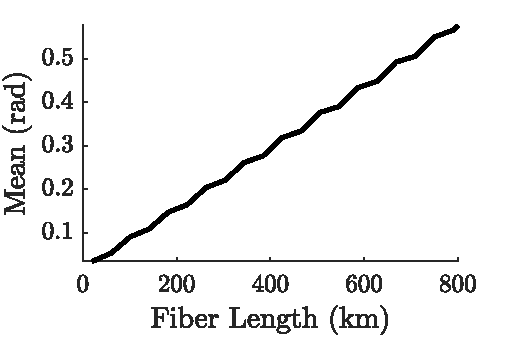
\includegraphics[width=0.5\linewidth]{img/APhiMean} & 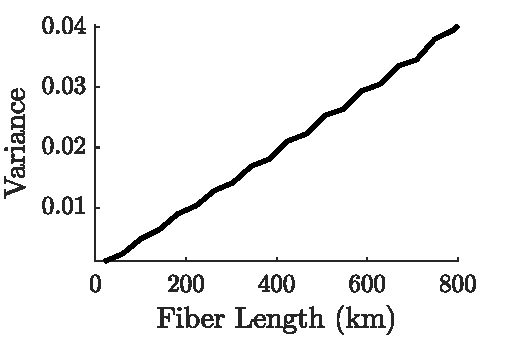
\includegraphics[width=0.5\linewidth]{img/APhiVar} \\
		(a) & (b)
	\end{tabular}
	\renewcommand{\baselinestretch}{1}
	\small\normalsize
	\caption{(a)\label{fig:APhiMean} Mean of $\phi$ vs. fiber length (b)\label{fig:APhiVar} Variance of $\phi$ vs. fiber length.}
\end{figure}
\renewcommand{\baselinestretch}{2}
\small\normalsize

The mean and variance of $\phi$ must also grow over the length of the fiber, but they no longer grow almost linearly because the data signal power varies. Instead, the mean and the variance grow in steps. Figures \ref{fig:APhiMean}a and \ref{fig:APhiVar}b show the mean and variance of $\phi$ respectively, in which flat regions where the data signal power is low are visible. The mean and variance are less than when attenuation was neglected because the average power of the data channels is lower.

%
\begin{figure}[htb]
	\raggedright
	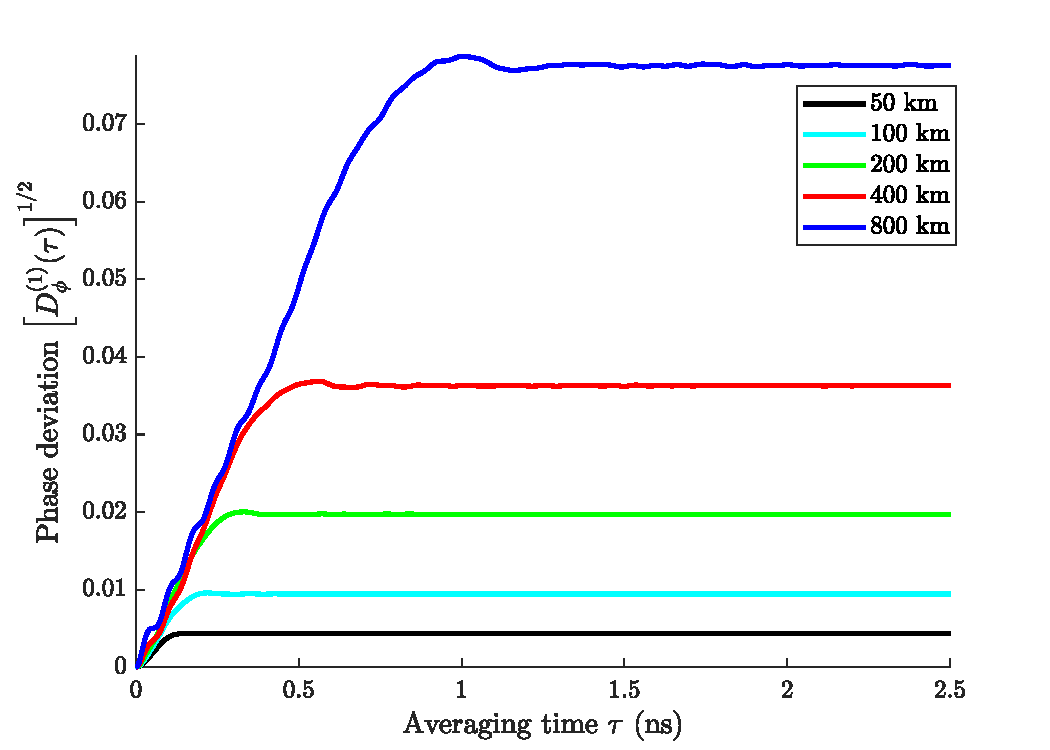
\includegraphics[scale=0.8]{img/APhaseStability}
	\renewcommand{\baselinestretch}{1}
	\small\normalsize
	\caption{Phase deviation with attenuation.} \label{fig:APhaseStability}
\end{figure}
\renewcommand{\baselinestretch}{2}
\small\normalsize%

The phase deviation $\left[D^{(1)}_\phi\right]^{1/2}$ reaches an asymptotic value as was the case when attenuation is neglected. Since the asymptotic value depends on the pulse spreading due to dispersion, the asymptotes occur at the same times. However, the phase deviation will be lower than was the case without attenuation, because the effect of XPM on the frequency signal from the data channels depends on the optical power of the data channels. Figure~\ref{fig:APhaseStability} shows $\left[D^{(1)}_\phi\right]^{1/2}$ for different fiber lengths.

Finally, the Allan deviation will be comparable to the results in the previous section. Figure~\ref{fig:AAllanDev} shows the Allan deviation for several fiber lengths, and we see a similar trend to what we saw without attenuation. At very low averaging times, $\tau < 10^{-11}$ s, there is higher uncertainty than in Figure~\ref{fig:NAAllanDev} due to high frequency ASE noise in the data signal. The Allan deviation will also decrease at a rate proportional to $\tau^{-1}$ after an averaging time interval approximately equal to the bit duration. We perform the same extrapolation as in the previous section, and we find an Allan deviation of $10^{-15}$ at $\tau=1$ s, and $10^{-18}$ at $\tau=10^3$ s.

\clearpage

%
\begin{figure}[htb]
	\raggedright
	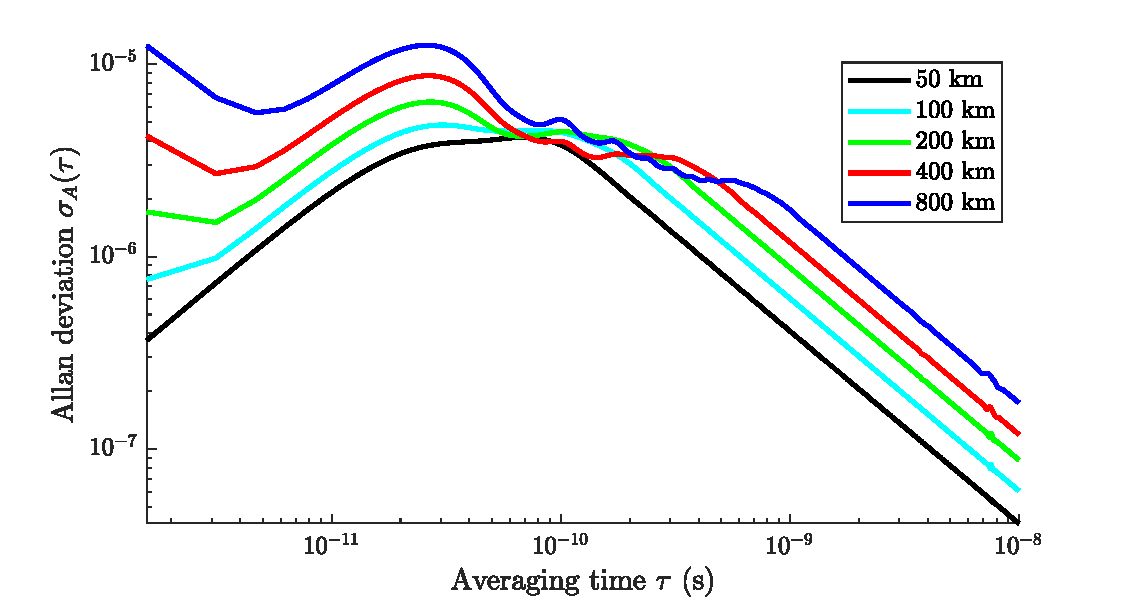
\includegraphics[scale=0.8]{img/AAllanDev}
	\renewcommand{\baselinestretch}{1}
	\small\normalsize
	\caption{Allan deviation with attenuation.} \label{fig:AAllanDev}
\end{figure}
\renewcommand{\baselinestretch}{2}
\small\normalsize%


\section{Varying the Frequency Separation}

The frequency separation between the data channels and the frequency signal will lead to a group velocity difference between the data channels and the signal channels, due to chromatic dispersion. The relative group velocity difference governs the rate at which the data signal travels through a fixed time point in the frequency signal. The group velocity difference is related to the separation between the center frequencies of the data channels and the frequency signal. The value $\delta = (v_{f}-v_{d})/(v_fv_d) = 1$ ps/km is chosen because it corresponds to placing the frequency signal at the midpoint between two neighboring data channels separated by $12.5$ GHz. As the separation between the center frequencies decreases, the group velocity difference decreases and thus $\delta$ decreases. 

Figure~\ref{fig:GVPhaseStability} shows the phase deviation for different frequency spacings between the data and frequency signal. The frequency separation in the figure refers to the separation between the center frequencies of the data channel and the frequency signal. The $6.25$ GHz separation refers to the system described in this thesis, where the frequency signal is placed in the boundaries of two closest neighboring data signals that conform with the ITU grid standard \cite{ITU-T2012}. The $12.5$ GHz separation corresponds to replacing a data channel with the frequency signal. Further separations are used to demonstrate the effect of XPM diminishing as the data channel is placed further away from the frequency signal.

\begin{figure}[htb]
	\raggedright
	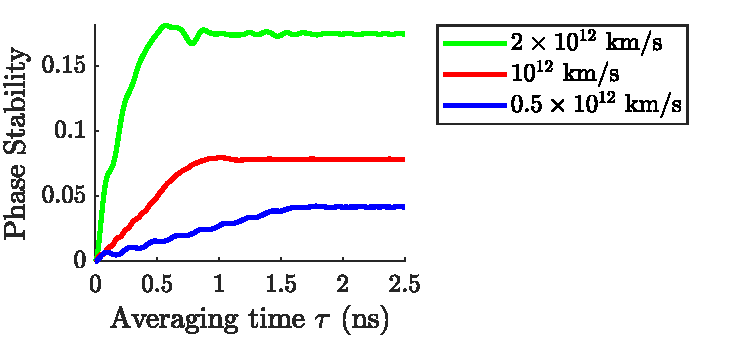
\includegraphics[scale=0.8]{img/GVPhaseStability}
	\renewcommand{\baselinestretch}{1}
	\small\normalsize
	\begin{quote}
		\caption{Phase deviation vs. group velocity difference.} \label{fig:GVPhaseStability}
	\end{quote}
\end{figure}
\renewcommand{\baselinestretch}{2}
\small\normalsize

\section{Comparison to Frequency Transfer Experiments}

Experiments in optical frequency transfer are typically performed on dark fibers or use frequencies alloted to a data channel. Experiments with simple unidirectional fiber optic links have an Allan deviation of $10^{-14}$ with one day of averaging \cite{UniExperiment1, UniExperiment2, UniExperiment3}. Improvements in frequency transfer have reduced the Allan deviation so that it is on the order of $10^{-17}$ with an averaging time of $10^5$ sec \cite{UniExperiment2,Experiment1}. Now, the primary source of phase noise in frequency transfer experiments is random temperature fluctuations over the length of the fiber \cite{TempExperiments}. 

Frequently these experiments are performed on optical fiber links that are in the range of $80$ -- $500$ km. The difference between the lengths of these experiments and our simulation is not a major concern, because the phase noise due to XPM increases as the length of the fiber link increases. We expect the larger distance in our simulations will exaggerate the phase noise due to XPM. Comparing the experiments to our results in the previous sections, we find that the phase noise due to XPM from placing the frequency signal in the interstices of two neighboring data channels is on the order of environmental effects.

\section{Chapter Remarks}

Since the bits in any data signal are uncorrelated, the phase deviation will asymptote after an averaging time that corresponds approximately to the time that it takes a single bit to slide through a constant phase point in the frequency signal. When the relative group velocity is greater, the phase deviation reaches its final value at a smaller distance because the data signal passes through a fixed time point in the frequency signal at a faster rate. 

The Allan deviation represents the expected frequency error. Experiments performing frequency transfer with a frequency signal that occupies an entire data channel on the ITU grid have Allan deviations that are comparable to our simulated values \cite{Serrano2013,cantin2017progress}. In this case, the frequency signal and data channels are separated by many GHz. The source of error in the experiments is environmental fluctuations. We have found that placing a frequency signal in the interstices of two data signals gives a frequency error on the order of environmental effects and should therefore be feasible. Hence, it is not necessary to use an entire data channel to transfer a frequency signal.